\documentclass[runningheads]{llncs}
\usepackage[T1]{fontenc}
\usepackage{amsmath,amssymb}
\usepackage{graphicx}
\usepackage{booktabs}
\usepackage{tabularx}
\usepackage{multirow}
\usepackage{xcolor}
\usepackage{hyperref}
\hypersetup{colorlinks=true,linkcolor=blue!50!black,citecolor=blue!50!black,urlcolor=blue!50!black}
\renewcommand\UrlFont{\color{blue}\rmfamily}

% ---------------------------------------------------------------
% Pending-result slots. Every \pending{ID}{...} is a task in
% todo-list.tex. Set \finaltrue to make compilation fail while any
% slot remains, which guarantees no placeholder reaches EasyChair.
% ---------------------------------------------------------------
\newif\iffinal
\finalfalse
\newcommand{\pending}[2]{\iffinal\errmessage{Unresolved pending result #1}\else{\color{red}[#1: #2]}\fi}
% Revision marking: blue only in the marked copy (main_marked.tex defines \MARKREV).
\newif\ifmarkrev
\ifdefined\MARKREV\markrevtrue\else\markrevfalse\fi
\newcommand{\rev}[1]{\ifmarkrev{\color{blue}#1}\else#1\fi}
\newcommand{\pendcell}[1]{\iffinal\errmessage{Unresolved pending result #1}\else{\color{red}[#1]}\fi}

\newcommand{\hd}[1]{{\bfseries\boldmath #1}}
\usepackage{etoolbox}
\AtBeginEnvironment{table}{\setlength{\belowcaptionskip}{4pt}}
\newcommand{\Hs}{\mathsf{H}}
\newcommand{\cG}{c_{G}}
\newcommand{\RC}{R_{C}}
\newcommand{\rhoo}{\rho_{\mathrm{old}}}
\newcommand{\rhon}{\rho_{\mathrm{new}}}
\newcommand{\Rel}{\mathcal{R}_{\mathsf{EUDR}}}
\newcommand{\Repoch}{\mathcal{R}_{\mathsf{epoch}}}

\setlength{\emergencystretch}{1.5em}
\renewcommand{\topfraction}{0.9}
\renewcommand{\textfraction}{0.08}
\renewcommand{\floatpagefraction}{0.85}
\setcounter{topnumber}{3}
\begin{document}

\title{Privacy-Preserving, Publicly Verifiable EUDR Compliance over EPCIS Event Data with Recursive Zero-Knowledge Proofs}
\titlerunning{Verifiable EUDR Compliance over EPCIS with Recursive ZK Proofs}

\author{Tuan-Dung Tran\inst{1,2}\thanks{Corresponding author.} \and
Van-Thinh Ngo\inst{1,2} \and
Huu-Tri Phan\inst{1,2} \and
Duy-Nhan Tran\inst{1,2}}
\authorrunning{T.-D. Tran et al.}
\institute{University of Information Technology, Ho Chi Minh City, Vietnam \and
Vietnam National University, Ho Chi Minh City, Vietnam\\
\email{dungtrt@uit.edu.vn}}

\maketitle

\begin{abstract}
The European Union (EU) Deforestation Regulation (EUDR) obliges operators to show, lot by lot, that coffee, cocoa, timber and four other commodities were not produced on land deforested after 31 December 2020. The plot coordinates and certificates that prove this are commercially sensitive: permissioned ledgers hide them from outside auditors, and public hash anchors prove nothing checkable. We present ZK-EUDR, a compliance protocol that turns Electronic Product Code Information Services (EPCIS) 2.0 events into a zero-knowledge relation with five predicates: geofence exclusion, credential membership, sensor threshold with time order, signer authorisation and a single-claim nullifier. Raw events stay on Hyperledger Fabric; each lot is proven in the SP1 zero-knowledge virtual machine, lot proofs are aggregated recursively into one Groth16 proof per epoch, and an Ethereum Virtual Machine (EVM) contract advances a nullifier-set root only after that proof verifies, so the on-chain cost of an epoch does not grow with its number of lots. We establish settlement soundness, with a proof sketch, under three binding conditions that we derive from the protocol. In an end-to-end run from Fabric to EVM settlement, the open-source implementation produced a 356-byte proof accepted for 293,364 gas and rejected a tampered proof, tampered public values and a replayed epoch. \pending{T-ABS-01}{one sentence with headline E2 latency (median/P95) and E3 gas-per-shipment ratio versus the three baselines} ZK-EUDR shows that regulatory traceability data can be governed as a verifiable, privacy-preserving database rather than disclosed.
\keywords{Zero-knowledge proofs \and Data governance \and Supply-chain traceability \and EPCIS \and EU Deforestation Regulation \and Recursive SNARKs \and Blockchain.}
\end{abstract}

% =================================================================
\section{Introduction}
\label{sec:intro}

Regulation (EU) 2023/1115, the EU Deforestation Regulation (EUDR), requires operators that place cattle, cocoa, coffee, oil palm, rubber, soya or wood on the EU market to file a due-diligence statement. The statement must give the geolocation of every production plot and show that the plot was not deforested after 31 December 2020~\cite{eudr2023}. After two postponements, the obligations apply from 30 December 2026 to large operators and from 30 June 2027 to micro and small enterprises~\cite{eudr2025amend}. EUDR compliance is therefore a data-integration problem: lot-level evidence is produced by many independent parties along a corridor and must be verifiable by a party outside it.

The information involved has traditionally been treated as a competitive asset. Farm coordinates, intermediary margins and certification audits reveal sourcing networks, and smallholder cooperatives in particular bear the cost of exposing them~\cite{zhunusova2022eudr}. Industrial traceability converges on GS1 Electronic Product Code Information Services (EPCIS) 2.0~\cite{gs1epcis2} for event capture and on a permissioned ledger such as Hyperledger Fabric~\cite{androulaki2018fabric} for cross-organisational sharing~\cite{saberi2019blockchain,behnke2020boundary}. This arrangement fails in the EUDR setting for two reasons: the competent authority and the importer sit outside the consortium, so granting them read access discloses the raw events, and the consortium can rewrite history before an audit without cryptographic detection. Anchoring event hashes on a public chain removes the second problem but not the first, because a hash means nothing without its preimage.

Zero-knowledge (ZK) proofs resolve this tension in principle. They have been applied to supply-chain provenance~\cite{sahai2020zkp,malik2022privchain}, to regulatory compliance on Fabric~\cite{yang2025zkfabledger}, to cross-chain token transfer between consortium and public chains~\cite{ding2026vecrotoken}, to mineral provenance with limited disclosure~\cite{hrabar2027oreproof}, and to location claims~\cite{ernstberger2025zklp}. \rev{Closest to this work, Ocean DPP proves Groth16 compliance predicates over EPCIS 2.0 sensor events for maritime product passports and batches their anchors in a Merkle tree~\cite{khairy2026oceandpp}. None of these works proves an EUDR-specific geospatial policy, aggregates per-lot proofs recursively into one proof, and settles that proof on a public chain through a nullifier state machine whose soundness conditions are stated.} What is missing is a compliance object that is derived from the events the industry already records, proves the regulatory predicate without revealing its inputs, has an on-chain cost independent of the number of lots per settlement period, and comes with soundness conditions precise enough to audit.

This paper addresses that problem from the data-governance side: EUDR compliance is treated as a verifiable predicate over a distributed event database. The contributions are as follows.
\begin{enumerate}
\item We formalise EUDR lot compliance as a relation $\Rel$ over a canonical 86-byte record derived from EPCIS 2.0 events, combining geofence exclusion, credential membership, threshold with time order, Ed25519 authorisation and a nullifier update, and we define an epoch relation $\Repoch$ that chains lots through nullifier roots.
\item We design ZK-EUDR, a settlement protocol that proves $\Rel$ per lot in the SP1 zero-knowledge virtual machine (zkVM)~\cite{sp1}, aggregates lot proofs recursively with fan-in eight and settles one Groth16 proof~\cite{groth2016} per epoch on an Ethereum Virtual Machine (EVM) contract, and we complement it with Plonky3 algebraic intermediate representations (AIRs)~\cite{plonky3} that cost each predicate.
\item We show, with a proof sketch, that an accepted epoch implies compliant witnesses for every aggregated lot and fresh nullifiers, under three binding conditions on registry roots, nullifier keys and commitment hiding.
\item We implement the protocol as open source, validate it end to end from Fabric to the EVM with tamper tests, and specify a paired evaluation with 30 seeds and Wilcoxon tests against Fabric-only, hash-on-chain and an adapted VeCroToken baseline.
\end{enumerate}

The rest of the paper is organised as follows. Section~\ref{sec:related} reviews related work and Section~\ref{sec:model} defines the system, data and threat models. Section~\ref{sec:design} presents the design, Section~\ref{sec:security} its security analysis and Section~\ref{sec:eval} the evaluation. Section~\ref{sec:discussion} discusses scope and Section~\ref{sec:conclusion} concludes.

% =================================================================
\section{Related Work}
\label{sec:related}

\subsubsection{EPCIS and ledger-based traceability.}
Blockchain traceability has been analysed for its effect on sustainable supply-chain management~\cite{saberi2019blockchain} and for the conditions under which partners share data~\cite{behnke2020boundary}. Hybrid EPCIS keeps GS1 events off-chain and anchors their digests on a ledger~\cite{tolcha2025hybrid}. Blockchain-based digital product passports follow a similar pattern~\cite{abreu2025dpp}. Fabric is the usual permissioned substrate~\cite{androulaki2018fabric}. These systems provide integrity among members but give an outside verifier either raw data or opaque hashes.

\subsubsection{Zero-knowledge supply-chain provenance.}
Sahai et al.\ use zero-knowledge succinct non-interactive arguments of knowledge (zk-SNARKs) to hide product transfers while preserving traceability~\cite{sahai2020zkp}. PrivChain proves location ranges and provenance claims to buyers without revealing the underlying data~\cite{malik2022privchain}. ProChain relies on encryption rather than public verifiability~\cite{li2024prochain}. zkFabLedger adds ZK-based regulatory compliance to Fabric transactions but keeps verification inside the permissioned network~\cite{yang2025zkfabledger}. VeCroToken moves zk-SNARK-verified tokens from consortium chains to a public chain~\cite{ding2026vecrotoken}, and OreProof combines Groth16 selective disclosure with Merkle-batched anchoring for gold provenance~\cite{hrabar2027oreproof}. \rev{Ocean DPP is the first system we know of that consumes EPCIS 2.0 events and proves threshold predicates over them with Groth16, settling Merkle-batched anchors on IOTA~\cite{khairy2026oceandpp}. Its batching aggregates anchors rather than proofs, so verification cost still grows with the number of proofs, and it has no geospatial predicate. No system in this group targets the EUDR predicate or aggregates lot proofs recursively.}

\subsubsection{Proof systems, zkVMs and verifiable data.}
Groth16 gives constant-size proofs that are cheap to verify on the EVM~\cite{groth2016}, scalable transparent arguments of knowledge (STARKs) built on the Fast Reed--Solomon interactive oracle proof of proximity (FRI) avoid a trusted setup~\cite{bensasson2018fri}, and zkVMs such as SP1~\cite{sp1} prove ordinary programs with recursion, trading circuit efficiency for auditability~\cite{yang2026sokzkvm}. Poseidon2 is the usual arithmetisation-friendly hash~\cite{grassi2023poseidon2}, and rollup soundness has recently been formalised~\cite{chaliasos2025rollups}. On the location side, zkLP proves IEEE-754 region membership~\cite{ernstberger2025zklp}. Selective-disclosure mechanisms for verifiable credentials have been benchmarked systematically~\cite{buldini2025sd}. In databases, ZKSQL and PoneglyphDB prove SQL query results over committed tables~\cite{li2023zksql,gu2025poneglyphdb}. The present work can be read as a domain-specific verifiable query: one fixed compliance predicate over an append-only event store, settled publicly.

\begin{table}[t]
\centering
\caption{Positioning against the closest related systems ($\checkmark$ supported, $\circ$ partial, -- absent or not reported in the cited paper).}
\label{tab:related}
\scriptsize
\setlength{\tabcolsep}{3pt}
\begin{tabularx}{\textwidth}{@{}l*{5}{>{\centering\arraybackslash}X}@{}}
\toprule
\hd{System} & \hd{EPCIS input} & \hd{Geospatial predicate} & \hd{ZK privacy} & \hd{Recursive aggregation} & \hd{Public settlement} \\
\midrule
PrivChain 2022~\cite{malik2022privchain} & -- & $\circ$ & $\checkmark$ & -- & -- \\
Hybrid EPCIS 2025~\cite{tolcha2025hybrid} & $\checkmark$ & -- & -- & -- & $\circ$ \\
zkFabLedger 2025~\cite{yang2025zkfabledger} & -- & -- & $\checkmark$ & -- & -- \\
zkLP 2025~\cite{ernstberger2025zklp} & -- & $\checkmark$ & $\checkmark$ & -- & -- \\
\rev{Ocean DPP 2026~\cite{khairy2026oceandpp}} & $\checkmark$ & -- & $\checkmark$ & -- & $\checkmark$ \\
VeCroToken 2026~\cite{ding2026vecrotoken} & -- & -- & $\checkmark$ & -- & $\checkmark$ \\
OreProof 2027~\cite{hrabar2027oreproof} & -- & -- & $\checkmark$ & -- & $\checkmark$ \\
This work & $\checkmark$ & $\checkmark$ & $\checkmark$ & $\checkmark$ & $\checkmark$ \\
\bottomrule
\end{tabularx}
\end{table}

Table~\ref{tab:related} summarises the comparison. ZK-EUDR is the only system in the table that provides all five properties. What sets it apart is a nullifier-chained recursive settlement: lot proofs are folded into one epoch proof whose public root advances an on-chain nullifier set, under binding conditions stated explicitly in Section~\ref{sec:security}.

% =================================================================
\section{System, Data and Threat Model}
\label{sec:model}

\subsection{System model}
Producers, processors and exporters emit EPCIS events signed with Ed25519 keys~\cite{bernstein2012ed25519} enrolled in the consortium. A permissioned Fabric channel (layer L0) stores each canonical event with its SHA-256 digest; the chaincode rejects duplicates and malformed records. A prover (the exporter or a service provider) reads the committed events of each lot, proves them, and aggregates the leaves of an epoch. A public EVM contract (layer L1) holds the current nullifier root and accepts an epoch only if its aggregate proof verifies. Auditors and importers read L1 and receive selective openings off-chain. A registry authority publishes the roots used as public inputs: the root $\RC$ of valid credentials and the commitment $\cG$ to the forest-loss polygon set, for example one derived from global forest-change maps~\cite{hansen2013forest}.

\subsection{Data model}
Each EPCIS 2.0 event is normalised into a fixed-width record
\[
e = (\mathit{id}, \ell, \epsilon, t, r, \phi, \lambda, \kappa, \varrho, \mathit{pk}) \in \{0,1\}^{86\cdot 8},
\]
with 64-bit identifiers $\mathit{id}$, lot $\ell$ and epoch $\epsilon$, a millisecond timestamp $t$, a 32-bit scaled key performance indicator (KPI) reading $r$, WGS-84 latitude and longitude $\phi,\lambda$ in signed micro-degrees, a 64-bit certificate identifier $\kappa$, a role code $\varrho$ and a 32-byte Ed25519 public key $\mathit{pk}$. \rev{Micro-degrees match the EUDR requirement of at least six decimal digits for geolocation coordinates~\cite[Art.~2(28)]{eudr2023}, about 0.11~m of latitude, and keep C1 in exact integer arithmetic.} Table~\ref{tab:mapping} gives the mapping from EPCIS 2.0 fields\rev{; truncating \texttt{eventID} to 64 bits makes a collision likely only after about $2^{32}$ events, and the chaincode rejects duplicate identifiers}. The chaincode, both provers and the tests share this encoding, so an event hashes identically at every layer. The artefact currently covers object events. Aggregation and transformation events, which merge or convert lots, are not yet mapped (Section~\ref{sec:discussion}; \pending{T-DM-01}{EPCIS 2.0 JSON-LD mapper}).

\begin{table}[t]
\centering
\caption{Mapping of EPCIS 2.0 event fields to the canonical record.}
\label{tab:mapping}
\scriptsize
\setlength{\tabcolsep}{5pt}
\begin{tabular}{@{}ll@{\hspace{14pt}}ll@{}}
\toprule
\hd{EPCIS 2.0 field} & \hd{Record} & \hd{EPCIS 2.0 field} & \hd{Record} \\
\midrule
\texttt{eventID}, 64-bit hash & $\mathit{id}$ & \texttt{sensorElementList}, scaled & $r$ \\
\texttt{epcList}/\texttt{quantityList} (LGTIN) & $\ell$ & \texttt{readPoint} geo URI, $10^{-6}$\,deg & $\phi,\lambda$ \\
settlement-period index & $\epsilon$ & \texttt{certificationInfo} & $\kappa$ \\
\texttt{eventTime}, ms & $t$ & \texttt{bizStep}/\texttt{sourceList} & $\varrho$ \\
\multicolumn{2}{@{}l}{} & signer enrolled in Fabric membership & $\mathit{pk}$ \\
\bottomrule
\end{tabular}
\end{table}

\subsection{Threat model}
Five adversaries are considered. T1, a producer, misreports plot coordinates so that a plot inside a forest-loss area appears compliant. T2, a processor, claims the same lot twice or mixes non-compliant lots into compliant ones\rev{; mixing through aggregation and transformation events is covered only once those events are mapped}. T3, the prover, attempts to settle an epoch that no compliant witness supports\rev{; a prover that omits lots is discussed in Section~\ref{sec:security}}. T4, a subset of consortium members, rewrites L0 history after settlement. T5, an auditor or a competitor reading L1, tries to learn coordinates, certificates or volumes beyond what has been disclosed. We assume knowledge soundness of the SP1 STARK, its recursion and its Groth16 wrapper, collision resistance of SHA-256, and existential unforgeability under chosen-message attacks (EUF-CMA) of Ed25519. The physical truth of sensor readings and GPS fixes is out of scope; it requires attestation hardware or remote sensing at the source.

\subsection{Compliance relations}
We write $\Hs$ for domain-separated SHA-256 with tag $\text{tag}_\ast$, $G=(v_1,\dots,v_k)$ with $3\le k\le 32$ for a simple polygon in micro-degrees, $\cG=\Hs(\text{tag}_G,k,G)$ for its commitment, $\RC$ for the root of the credential tree, $\sigma_i$ and $\pi^C_i$ for the signature and credential path of $e_i$, $\tau$ and $\varrho^\star$ for the KPI threshold and the required role, $s$ for the nullifier secret of a lot, $\pi^N$ for its path in the depth-32 sparse nullifier tree, and $\rhoo,\rhon$ for that tree's roots before and after the update. The event-batch digest is $D=\Hs(\text{tag}_D,n,\mathsf{bytes}(e_1)\|\cdots\|\mathsf{bytes}(e_n))$.

\begin{definition}[EUDR lot relation]\label{def:rel}
For a statement $x$ and a witness $w$ of the form
\[
x=(\epsilon,\rhoo,\rhon,D,\RC,\cG,\nu,\varrho^\star,\tau,n),\qquad w=(\ell,G,(e_i,\sigma_i,\pi^C_i)_{i\le n},s,\pi^N),
\]
we have $(x,w)\in\Rel$ if and only if $8\le n\le 64$, $\cG=\Hs(\text{tag}_G,k,G)$, $D$ is the batch digest of $(e_i)$, and for every $i$:
\begin{description}
\item[C1] the point $(\phi_i,\lambda_i)$ lies strictly outside the simple polygon $G$;
\item[C2] $\mathsf{MerkleVerify}(\RC,\Hs(\text{tag}_C,i,\kappa_i,\mathit{pk}_i,\varrho_i),\pi^C_i)=1$;
\item[C3] $\ell_i=\ell$, $\epsilon_i=\epsilon$, $\varrho_i=\varrho^\star$, $r_i\le\tau$ and $t_i>t_{i-1}$ for $i>1$;
\item[C4] $\mathsf{Ed25519.Verify}(\mathit{pk}_i,\mathsf{bytes}(e_i),\sigma_i)=1$;
\item[C5] $\nu=\Hs(\ell,s)$ and, at index $j=\nu[0..32)$, the sparse tree with sibling path $\pi^N$ has root $\rhoo$ when leaf $j$ is empty and root $\rhon$ when leaf $j$ is marked used.
\end{description}
\end{definition}

\begin{definition}[Epoch relation]\label{def:epoch}
Child statements $(x_1,\dots,x_m)$, each a lot or an aggregate statement, satisfy $\Repoch$ with output $(\epsilon,\rho_0,\rho_m,\Gamma,L,N)$ if all have epoch $\epsilon$; the old root of child $j$ equals the new root of child $j-1$ and every child changes its root; child digests are pairwise distinct; aggregate children carry the expected leaf and aggregate verifying-key digests; $L$ and $N$ are the summed lot and event counts with $8L\le N\le 64L$; and $\Gamma$ is a hash over the ordered child digests, root pairs and counts.
\end{definition}

% =================================================================
\section{Design}
\label{sec:design}

\begin{figure}[t]
\centering
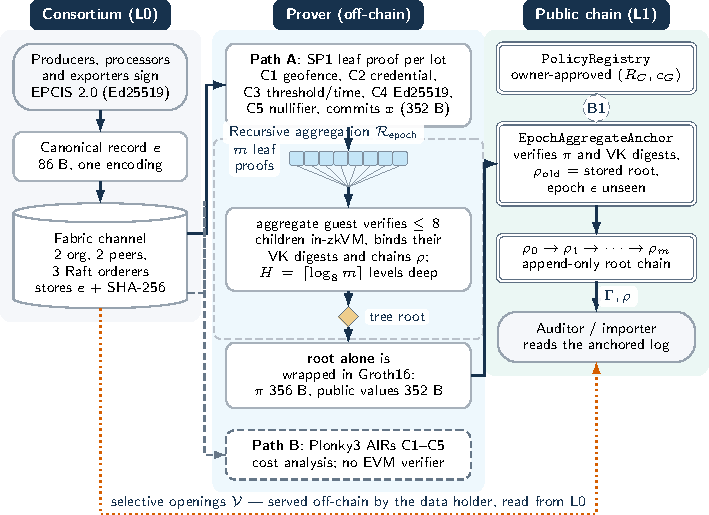
\includegraphics[width=0.94\textwidth]{figures/architecture.pdf}
\caption{Architecture. Canonical EPCIS records are committed on Fabric (L0). Path A proves $\Rel$ per lot in SP1, aggregates leaves into $\Repoch$ with fan-in eight, wraps the root in Groth16 and settles it on the EVM (L1). Path B proves each predicate as a Plonky3 AIR for cost analysis. Auditors check L1 and receive openings off-chain \rev{from the data holder, who reads them from L0}.}
\label{fig:arch}
\end{figure}

\subsection{Leaf proofs in a zkVM (Path A)}
Figure~\ref{fig:arch} shows the pipeline. The SP1 guest receives the serialised witness of one lot, decodes each event, checks C3, C1, C4 and C2 in turn while hashing the event into $D$, aborts on the first failure, and finally performs the C5 update and commits $x$. Every predicate is ordinary Rust code. C1 is an exact integer crossing-number test over micro-degrees that rejects points on an edge, so no floating-point arithmetic is involved. C2 and C5 use domain-separated SHA-256 Merkle trees, and C4 uses strict \texttt{ed25519-dalek} verification. The commitment is the 352-byte application binary interface (ABI) encoding of $x$. Writing the policy as a program rather than a circuit lets a regulator's engineers audit it in a mainstream language, at the cost of prover time~\cite{yang2026sokzkvm}.


The work per lot is $O(n(k+d_C))$ hash and arithmetic operations plus $n$ signature checks and $d_N=32$ hashes for C5, where $k$ is the number of polygon vertices and $d_C$ the credential depth. The leaf proof size does not depend on $n$\rev{, because the STARK is compressed and then wrapped in a constant-size Groth16 proof}.

\subsection{Recursive epoch aggregation}
A second guest program verifies up to eight child proofs with SP1's in-zkVM verifier, binding each child's hashed public values to the verifying-key digest of the leaf or aggregate program, and then evaluates $\Repoch$ (Definition~\ref{def:epoch}) and commits a 288-byte statement. For an epoch of $m$ lots, the aggregation tree has depth $H=\max(1,\lceil\log_8 m\rceil)$ and requires $\sum_{h=1}^{H}\lceil m/8^h\rceil\le\lceil(m-1)/7\rceil+H$ aggregation proofs. Lots larger than 64 events are split into several leaves. Only the root is wrapped in Groth16, so one epoch costs a single pairing-based verification on L1 for any $m$, whereas a per-lot design pays $m$.

\subsection{Settlement contract}
\texttt{EpochAggregateAnchor} calls the SP1 Groth16 verifier with the program key and then requires that the epoch is new, that the statement is valid with $8L\le N\le64L$, that its epoch and old root match both the caller's expectation and the stored root, and that both verifying-key digests equal the values fixed at deployment. Only then does it store $\rho_m$ and emit $(\epsilon,\Gamma,\rho_0,\rho_m,L,N)$. Since the root advances only through verified transitions, anchored epochs form an append-only public log of compliance claims, and a later rewrite of L0 (T4) changes some $D$ and hence conflicts with the anchored $\Gamma$.

\subsection{Per-predicate AIRs (Path B)}
\rev{Path B isolates the cost of the predicates from the cost of the zkVM, acting as a circuit-level lower bound for Path A.} C1 to C5 are Plonky3 AIRs over Goldilocks with Poseidon2 and FRI: a serial crossing-number AIR (C1), a depth-16 Poseidon2 Merkle path (C2), 32-bit range checks with time ordering (C3), a Poseidon2 authorisation preimage instead of Ed25519 (C4), and a depth-32 sparse-map update (C5). A recursive wrapper verifies and pairwise aggregates the five proofs. \rev{The two paths differ in hash function, credential depth and C4, so Path B numbers bound Path A from below only after these parameters are aligned \pending{T-E1-01}{rerun with Path A parameters}. Path B has no EVM verifier and is not used for settlement.}

\subsection{Selective-disclosure compliance view}
Public statements carry commitments, not data. A compliance view $\mathcal{V}$ is a set of openings handed to one auditor: the leaf statements of the relevant lots (which recompute $\Gamma$), the polygon $G$ for $\cG$, credential leaves for $\RC$, and the lot identifier with its secret for $\nu$. Views for different stakeholders differ only in their openings, and no proof is regenerated. Opening a subset of a lot's events requires replacing the sequential digest $D$ by a Merkle root over events, and the whole mechanism requires hiding commitments (Section~\ref{sec:security}); both are part of \pending{T-SD-01}{view prototype, opening size and verification time}.

% =================================================================
\section{Security Analysis}
\label{sec:security}

\begin{proposition}[Settlement soundness]\label{prop:sound}
Assume the proof system is knowledge-sound, SHA-256 is collision-resistant and Ed25519 is EUF-CMA secure. Suppose the contract accepts an epoch statement $(\epsilon,\rho_0,\rho_m,\Gamma,L,N)$, and suppose the binding conditions B1 to B3 below hold. Then, except with negligible probability, there exist $L$ witnesses satisfying $\Rel$ whose statements chain from $\rho_0$ to $\rho_m$. Every lot nullifier inserted is fresh with respect to all previously anchored epochs, and every event was signed by a key that holds a valid credential under the registered root.
\end{proposition}

\begin{proof}[sketch]
Step 1. By knowledge soundness of the Groth16 wrapper and of SP1 recursive composition \rev{with verifying-key-digest binding}, an accepting proof under the fixed program key yields an execution of the aggregate guest. That execution verified each child under the committed verifying-key digests, and the contract checks those digests, so by induction on the aggregation tree every leaf statement was produced by the leaf program on some witness. The leaf program aborts unless every predicate of Definition~\ref{def:rel} holds, so each witness satisfies $\Rel$. Step 2. $\Repoch$ chains consecutive roots and forces each to change, and the contract forces $\rho_0$ to equal the stored root, so the roots form a single path from the stored root. Inserting into a leaf that is already used would require two distinct paths to the same root, that is, a SHA-256 collision. Step 3. Under B1, $\RC$ is the registered root. Producing a valid leaf for an unenrolled key would require either a Merkle collision or a forged Ed25519 signature on $\mathsf{bytes}(e_i)$. \qed
\end{proof}

The proposition holds only together with three binding conditions. \rev{All measurements in Section~\ref{sec:eval} use the artefact before these fixes, which is stated with each result.}
\begin{description}
\item[B1 (registry binding)] $\RC$ and $\cG$ in each leaf must equal the registry's values; otherwise a T1/T3 adversary proves compliance against a self-chosen polygon or credential tree. The aggregate statement does not yet carry them and the contract does not check them. The fix propagates both values into $\Gamma$ and compares them with registry storage\rev{, adding 64 bytes of public values and two storage reads} \pending{T-SEC-01}{implemented and tested}.
\item[B2 (key-bound nullifiers)] With $\nu=\Hs(\ell,s)$ and a prover-chosen $s$, one lot can be claimed twice with two secrets (T2); $s$ must be derived from a key committed in the owner's credential leaf, as account nullifiers are bound to spending keys. The 32-bit index also collides after about $2^{16}$ lots, a liveness rather than a soundness fault that calls for a wider index\rev{, which multiplies the C5 hashing per lot by eight for a 256-level tree} (\pending{T-SEC-03}{key-bound nullifier and 256-bit index}).
\item[B3 (hiding commitments)] $\cG$ and $D$ are unsalted, so polygons from a public forest-loss map and low-entropy events fall to a dictionary attack (T5); a 256-bit nonce in the witness restores hiding (\pending{T-SEC-02}{salted commitments}).
\end{description}
\rev{The proposition concerns soundness, not completeness: a prover can omit lots committed on Fabric, which censors their claims but cannot make a non-compliant lot appear compliant. Binding each epoch to a committed range of Fabric blocks and proving coverage would close this gap.} For Path B, the FRI parameters used in the archived benchmark (blowup 4, 8 queries, no proof-of-work grinding) give only about 16 bits of conjectured security~\cite{bensasson2018fri}. Those measurements show how cost scales and are not a deployable configuration (Section~\ref{sec:eval}).

% =================================================================
\section{Evaluation}
\label{sec:eval}

\subsection{Research questions and protocol}
Research question RQ1 asks what each predicate and each leaf costs as $n$ grows; RQ2, what audit latency the pipeline achieves from the Fabric acknowledgement of a lot's last event to the L1 receipt; RQ3, how the design compares with three baselines in throughput, gas, calldata and latency; and RQ4, how it scales with the number of producers $N_p$, the shipment size and the epoch length.

The ChaCha20-seeded synthetic workload has $N_p=125$ producers emitting Poisson arrivals at 3.84 events per minute each (480 events per minute) for 60 minutes, with lots of 8 to 64 events and 60~s epochs. Each configuration runs for 30 paired seeds, with mode order rotated per seed\rev{ and the Fabric ledger and Anvil state reset before each run, so that ledger growth does not confound the modes}. Results are reported as median, interquartile range (IQR), 95th percentile (P95) and a 10,000-resample bootstrap 95\% confidence interval. Pairwise comparisons use the exact Wilcoxon signed-rank test with Bonferroni correction over six pairs and Cliff's $\delta$ as the effect size. Censored and saturated runs are reported and never dropped\rev{; RQ4 is analysed descriptively, without hypothesis tests}. RQ3 compares four modes on identical events: Fabric-only makes no L1 transaction; hash-on-chain anchors one SHA-256 digest per shipment; VeCroToken-adapted verifies one SP1 policy proof and records a token mint per leaf; and the proposed mode settles one aggregate proof per epoch. This adapter reuses our policy statement and does not reproduce VeCroToken's cross-chain or attribute-encryption protocol~\cite{ding2026vecrotoken}\rev{, so it is an ablation of recursive aggregation rather than a reproduction}. RQ4 runs a screening grid of 80 cells with $N_p\in\{125,250,500,1000,2000\}$, shipment size $\in\{16,32,64,128\}$ and epoch length $\in\{30,60,120,300\}$~s, followed by a confirmation grid of 27 cells with 10 seeds each.

\subsection{Implementation and setup}
The artefact\footnote{\url{https://github.com/vanthinh26102005/nckh-ise-blockchain}} uses Plonky3 0.6 (recursion at \texttt{b363397}), SP1 SDK 6.4.0 with Groth16 verifier v6.1.0, Fabric 2.5.8 with Go chaincode and a commit-waiting Gateway, Solidity 0.8.20 and Anvil. Formal runs use two organisations, two peers and three Raft orderers, with proving on an NVIDIA A100 after a recorded CPU/GPU preflight (\pending{T-E2-01}{3-Raft topology and host specification}). The archived Path B benchmark ran on an 8-core Apple-silicon laptop.

\subsection{Functional validation (measured)}
One complete run exercised every layer (Table~\ref{tab:e2smoke}). Eight canonical events of one lot were written through the Fabric Gateway, endorsed by both organisations of a two-peer, one-orderer network, and read back. An SP1 Groth16 proof of $\Rel$ was generated and verified locally, and \texttt{EpochAnchor} accepted it on Anvil, while a proof with one byte changed, public values with one byte changed and a replayed epoch were all rejected. A recursive Path B test that proves and verifies all five AIRs also passes; it took about 782~s and has not been benchmarked.

\begin{table}[t]
\centering
\caption{Measured end-to-end run, Fabric to SP1 to EVM (one lot, $n=8$, CPU prover on the development workstation, single run, \rev{artefact before the B1--B3 fixes}).}
\label{tab:e2smoke}
\scriptsize
\begin{tabular}{@{}lr@{}}
\toprule
\hd{Quantity} & \hd{Value} \\
\midrule
Events written and read back through Fabric & 8 / 8 \\
SP1 Groth16 proving time after Fabric acknowledgement & 842.9 s \\
Contract deployment and anchoring step on Anvil & 3.2 s \\
Fabric acknowledgement to L1 receipt & 846.1 s \\
Proof size / ABI public values & 356 B / 352 B \\
Gas of the accepted \texttt{verifyAndAnchor} transaction & 293,364 \\
Tampered proof / tampered public values / replayed epoch & all rejected \\
\bottomrule
\end{tabular}
\end{table}

\subsection{RQ1: predicate and leaf cost}
Table~\ref{tab:rq1} reports archived Path B measurements for C2 to C5 over 30 seeds per cell. Proving time for C3 grows linearly with $n$ (1.13~ms to 7.92~ms) and its proof grows from 11.1 to 19.0~kB, because the trace has one row group per event. C2, C4 and C5 prove one path or preimage per lot and are flat in $n$. \rev{The 95\% bootstrap half-widths are below 6\% of the mean except for C2 at $n=64$ and the verification times of C2 at $n=8$ and C5 at $n=64$, which range from 13\% to 31\% because of a few outlier runs.} The Merkle-based AIRs (C2, C5) dominate proof size at about 276~kB because each of their 16 or 32 levels is a Poseidon2 permutation. These older circuit versions ran at about 16-bit FRI security, so Table~\ref{tab:rq1} reserves rows for the production rerun, including C1, the wrapper and the SP1 leaf.

\begin{table}[t]
\centering
\caption{RQ1. Path B per-predicate cost: mean over 30 seeds (archived, 8-core Apple silicon, about 16-bit FRI security), plus pending production rows.}
\label{tab:rq1}
\scriptsize
\setlength{\tabcolsep}{4pt}
\begin{tabular}{@{}lrrrrrr@{}}
\toprule
& \multicolumn{3}{c}{\hd{$n=8$}} & \multicolumn{3}{c}{\hd{$n=64$}} \\
\cmidrule(lr){2-4}\cmidrule(lr){5-7}
\hd{Predicate} & \hd{Prove} & \hd{Verify} & \hd{Proof} & \hd{Prove} & \hd{Verify} & \hd{Proof} \\
 & \hd{(ms)} & \hd{(ms)} & \hd{(kB)} & \hd{(ms)} & \hd{(ms)} & \hd{(kB)} \\
\midrule
C2 Merkle, depth 16 & 10.4 & 11.5 & 275.5 & 12.9 & 11.2 & 275.7 \\
C3 threshold and time & 1.13 & 0.53 & 11.1 & 7.92 & 0.77 & 19.0 \\
C4 auth.\ (Poseidon2) & 0.40 & 0.44 & 11.7 & 0.41 & 0.44 & 11.7 \\
C5 nullifier (empty leaf) & 10.4 & 10.4 & 276.2 & 10.6 & 11.2 & 276.2 \\
\midrule
C1--C5 at $\ge$100-bit FRI & \multicolumn{6}{c}{\pending{T-E1-01}{production-parameter rerun}} \\
Recursive wrapper (B) & \multicolumn{6}{c}{\pending{T-E1-02}{time and size}} \\
SP1 leaf, CPU/GPU (A) & \multicolumn{6}{c}{\pending{T-E1-03}{leaf time, proof sizes}} \\
\bottomrule
\end{tabular}
\end{table}

\subsection{RQ2: audit latency}
In the measured run, 99.6\% of the 846.1~s audit latency is CPU proving and 0.4\% is L1 settlement (Table~\ref{tab:e2smoke}). The latency of the design is therefore governed by prover throughput, not by the ledgers. This is why the formal configuration proves on a GPU and parallelises leaves within an epoch. \rev{Parallel leaf proving is possible although the nullifier roots chain sequentially, because the host computes every sparse-tree path of the epoch before proving starts, so each leaf receives its old root as input.} The distribution over the full workload is \pending{T-E2-02}{median, P95, P99 over 30 seeds at 480 events/min}.

\subsection{RQ3: comparison with baselines}
With $G_v\approx2.93\times10^5$ gas measured for verifying and anchoring one Groth16 policy proof (Table~\ref{tab:e2smoke}), an epoch of $m$ lots costs about $mG_v$ in the VeCroToken-adapted mode but one aggregate verification $G_a$ in the proposed mode, so settlement cost per shipment should fall by about $m\,G_v/G_a$ while aggregation moves off-chain. Hash-on-chain and Fabric-only give strictly weaker guarantees, \rev{which Table~\ref{tab:rq3} records next to each mode so that throughput is not compared across security levels}. Its cells are reserved until the gate of the recursive epoch proof, an Anvil receipt for a two-lot aggregate, has passed and all 120 runs have completed.

\begin{table}[t]
\centering
\caption{RQ3. Paired comparison on identical workloads (median [IQR] over 30 seeds).}
\label{tab:rq3}
\scriptsize
\setlength{\tabcolsep}{2.4pt}
\begin{tabular}{@{}llcccc@{}}
\toprule
\hd{Mode} & \hd{\rev{Public guarantee}} & \hd{Throughput} & \hd{Gas per} & \hd{Calldata per} & \hd{Audit} \\
 & & \hd{(lots/min)} & \hd{shipment} & \hd{shipment (B)} & \hd{latency (s)} \\
\midrule
Fabric-only & \rev{none} & \pendcell{T-E3-02} & n/a & n/a & \pendcell{T-E3-02} \\
Hash-on-chain & \rev{digest only} & \pendcell{T-E3-02} & \pendcell{T-E3-02} & \pendcell{T-E3-02} & \pendcell{T-E3-02} \\
VeCroToken-adapted & \rev{ZK, per lot} & \pendcell{T-E3-02} & \pendcell{T-E3-02} & \pendcell{T-E3-02} & \pendcell{T-E3-02} \\
Proposed & \rev{ZK, per epoch} & \pendcell{T-E3-02} & \pendcell{T-E3-01} & \pendcell{T-E3-02} & \pendcell{T-E3-02} \\
\bottomrule
\end{tabular}
\end{table}

\subsection{RQ4: scalability and policy trade-offs}
RQ4 measures throughput, completion rate, leaf and aggregate proving time, audit latency, gas and calldata over the screening and confirmation grids. Gas is converted to fiat cost with a documented gas price and exchange rate (\pending{T-COST-01}{conversion script and assumptions}). Screening results (\pending{T-E4-01}{80 runs}) select the region shown in Fig.~\ref{fig:rq4}.

\begin{figure}[t]
\centering
\fbox{\parbox[c][34mm][c]{0.92\textwidth}{\centering\pending{T-E4-02}{two-panel PGFPlots figure from the 270 confirmation runs: (a) throughput and completion rate, (b) gas and calldata per shipment, versus shipment size and epoch length}}}
\caption{RQ4. Scalability of the proposed design over the confirmation grid (median and IQR over 10 seeds per cell; censored cells marked).}
\label{fig:rq4}
\end{figure}

% =================================================================
\section{Discussion and Limitations}
\label{sec:discussion}

Path A settles on the EVM with auditable Rust and real Ed25519 signatures but proves slowly; Path B costs predicates without an EVM verifier, and the two are never mixed in one table. \rev{The main threat to validity is the fidelity of C1 to the regulation. EUDR describes plots of more than four hectares by polygons~\cite[Art.~2(28)]{eudr2023}, and a plot polygon can overlap forest loss while its sampled points do not. A faithful predicate therefore tests polygon disjointness against every forest-loss polygon of a map tile, with a proof that the tile list is complete under the registered root} (\pending{T-C1-01}{plot-polygon and multi-polygon C1}). Further limitations are as follows. First, aggregation and transformation events are not yet mapped; treating them as edges of a lot graph and proving continuity over that graph is the natural extension. Second, results on Anvil reflect EVM execution and not network inclusion delay (\pending{T-SEP-01}{optional public-testnet run}). Third, B1 to B3 must be enforced before deployment. Finally, the physical truth of GPS fixes and sensor readings depends on attestation at the source. \rev{Two societal risks also deserve mention. Smallholders who cannot produce signed, geotagged events may be excluded from EU supply chains~\cite{zhunusova2022eudr}, so onboarding through cooperatives matters as much as cryptography. In addition, the registry authority that publishes $\RC$ and $\cG$ becomes a point of control and should itself be auditable.}

For databases, the design suggests a pattern: an append-only, multi-writer event store whose compliance predicate is proven once per epoch and settled publicly, with openings served on demand. ZKSQL and PoneglyphDB prove arbitrary queries over one committed table~\cite{li2023zksql,gu2025poneglyphdb}; here the predicate is fixed, the writers distrust each other and the verifier is a contract. Proving ad hoc auditor queries over the anchored commitments would combine the two.

% =================================================================
\section{Conclusion}
\label{sec:conclusion}

This paper proposed ZK-EUDR, a protocol that proves EUDR lot compliance in zero knowledge over EPCIS-derived records, aggregates lot proofs recursively and settles one Groth16 proof per epoch on an EVM contract that maintains a nullifier-set root. Its formal relations make the compliance predicate auditable, its settlement-soundness proposition names the binding conditions under which an accepted epoch implies compliance, and an end-to-end Fabric-to-EVM run confirmed the path with a 356-byte proof settled for 293,364 gas while tampered inputs were rejected. \pending{T-ABS-01}{headline RQ2/RQ3 findings}

Future work will extend C1 from points to plot polygons tested against every forest-loss polygon of a registered map tile, prove continuity over the lot graph induced by aggregation and transformation events, and pilot the protocol with a Vietnamese coffee cooperative and an EU importer. The same predicate structure also fits the Carbon Border Adjustment Mechanism and digital product passports~\cite{abreu2025dpp}.

\begin{credits}
\subsubsection{\ackname} \pending{T-DOC-01}{funding acknowledgement and ORCID identifiers}
\subsubsection{\discintname} The authors have no competing interests to declare that are relevant to the content of this article.
\end{credits}

% Bibliography embedded from main.bbl (generated with splncs04 from references.bib).
\begin{thebibliography}{10}
\providecommand{\url}[1]{\texttt{#1}}
\providecommand{\urlprefix}{URL }
\providecommand{\doi}[1]{https://doi.org/#1}

\bibitem{abreu2025dpp}
Abreu, H., Pereira, V., Barata, J.: Blockchain-based digital product passport:
  design principles and demonstration. International Journal of Production
  Research  \textbf{63},  5863--5882 (2025).
  \doi{10.1080/00207543.2025.2464161}

\bibitem{androulaki2018fabric}
Androulaki, E., Barger, A., Bortnikov, V., Cachin, C., et~al.: Hyperledger
  {Fabric}: A distributed operating system for permissioned blockchains. In:
  Proc. 13th EuroSys Conference. pp. 1--15 (2018).
  \doi{10.1145/3190508.3190538}

\bibitem{behnke2020boundary}
Behnke, K., Janssen, M.: Boundary conditions for traceability in food supply
  chains using blockchain technology. International Journal of Information
  Management  \textbf{52},  101969 (2020).
  \doi{10.1016/j.ijinfomgt.2019.05.025}

\bibitem{bensasson2018fri}
Ben-Sasson, E., Bentov, I., Horesh, Y., Riabzev, M.: Fast {Reed-Solomon}
  interactive oracle proofs of proximity. In: Proc. 45th Int. Colloquium on
  Automata, Languages, and Programming (ICALP). LIPIcs, vol.~107, pp.
  14:1--14:17 (2018). \doi{10.4230/LIPIcs.ICALP.2018.14}

\bibitem{bernstein2012ed25519}
Bernstein, D.J., Duif, N., Lange, T., Schwabe, P., Yang, B.Y.: High-speed
  high-security signatures. Journal of Cryptographic Engineering
  \textbf{2}(2),  77--89 (2012). \doi{10.1007/s13389-012-0027-1}

\bibitem{buldini2025sd}
Buldini, A., Mazzocca, C., Montanari, R., Uluagac, S.: Benchmarking selective
  disclosure mechanisms for verifiable credentials: A systematic comparison for
  security and privacy. IEEE Transactions on Information Forensics and Security
   \textbf{20},  13205--13220 (2025). \doi{10.1109/TIFS.2025.3636051}

\bibitem{chaliasos2025rollups}
Chaliasos, S., Firsov, D., Livshits, B.: Towards a formal foundation for
  blockchain {ZK} rollups. In: Proc. ACM SIGSAC Conf. on Computer and
  Communications Security (CCS). pp. 2714--2728 (2025).
  \doi{10.1145/3719027.3765115}

\bibitem{ding2026vecrotoken}
Ding, K., Hu, X., Zhou, W., Cheng, G., Li, R.: {VeCroToken}: An efficient,
  verifiable, and privacy-preserving cross-chain model for consortium
  blockchains based on {zk-SNARKs}. IEEE Transactions on Network and Service
  Management  \textbf{23},  1543--1558 (2026). \doi{10.1109/TNSM.2025.3636014}

\bibitem{ernstberger2025zklp}
Ernstberger, J., Zhang, C., Ciprian, L., Jovanovic, P., Steinhorst, S.:
  Zero-knowledge location privacy via accurate floating-point {SNARKs}. In:
  Proc. IEEE Symposium on Security and Privacy (SP). pp. 3440--3459 (2025).
  \doi{10.1109/SP61157.2025.00057}

\bibitem{eudr2023}
{European Parliament and Council of the European Union}: Regulation ({EU})
  2023/1115 on deforestation-free products. Official Journal of the European
  Union, L 150, pp. 206--247 (2023),
  \url{https://eur-lex.europa.eu/eli/reg/2023/1115/oj}

\bibitem{eudr2025amend}
{European Parliament and Council of the European Union}: Regulation ({EU})
  2025/2650 amending {Regulation (EU) 2023/1115} as regards its date of
  application and simplification. Official Journal of the European Union, 23
  Dec. 2025 (2025), \url{https://eur-lex.europa.eu/eli/reg/2025/2650/oj}

\bibitem{grassi2023poseidon2}
Grassi, L., Khovratovich, D., Schofnegger, M.: {Poseidon2}: A faster version of
  the {Poseidon} hash function. In: Progress in Cryptology -- AFRICACRYPT 2023.
  pp. 177--203. LNCS, Springer (2023). \doi{10.1007/978-3-031-37679-5_8}

\bibitem{groth2016}
Groth, J.: On the size of pairing-based non-interactive arguments. In: Advances
  in Cryptology -- EUROCRYPT 2016. LNCS, vol.~9666, pp. 305--326. Springer
  (2016). \doi{10.1007/978-3-662-49896-5_11}

\bibitem{gs1epcis2}
{GS1}: {EPCIS} and {CBV} 2.0 standard. Tech. rep., GS1 AISBL, Brussels (2022),
  \url{https://ref.gs1.org/standards/epcis/}

\bibitem{gu2025poneglyphdb}
Gu, B., Fang, J., Nawab, F.: {PoneglyphDB}: Efficient non-interactive
  zero-knowledge proofs for arbitrary {SQL}-query verification. Proceedings of
  the ACM on Management of Data  \textbf{3}(1),  1--27 (2025).
  \doi{10.1145/3709713}

\bibitem{hansen2013forest}
Hansen, M.C., Potapov, P.V., Moore, R., Hancher, M., Turubanova, S.A.,
  Tyukavina, A., et~al.: High-resolution global maps of 21st-century forest
  cover change. Science  \textbf{342}(6160),  850--853 (2013).
  \doi{10.1126/science.1244693}

\bibitem{hrabar2027oreproof}
Hrabar, O., Soufiani, H.A., Kim, H.M.: {OreProof}: Verifiable provenance with
  limited disclosure for critical-minerals supply chains using zero-knowledge
  proofs. In: Proc. 60th Hawaii Int. Conf. on System Sciences (HICSS-60), to
  appear (2027). \doi{10.48550/arXiv.2609.00340}, arXiv:2609.00340

\bibitem{khairy2026oceandpp}
Khairy, S., Falcitelli, M.: A {DLT}- and {ZKP}-enabled framework for
  privacy-preserving digital product passports in maritime container logistics.
  Logistics  \textbf{10}(8) (2026). \doi{10.3390/logistics10080177}

\bibitem{li2024prochain}
Li, J., Wang, Z., Guan, S., Cao, Y.: {ProChain}: A privacy-preserving
  blockchain-based supply chain traceability system model. Computers \&
  Industrial Engineering  \textbf{187},  109831 (2024).
  \doi{10.1016/j.cie.2023.109831}

\bibitem{li2023zksql}
Li, X., Weng, C., Xu, Y., Wang, X., Rogers, J.: {ZKSQL}: Verifiable and
  efficient query evaluation with zero-knowledge proofs. Proceedings of the
  VLDB Endowment  \textbf{16}(8),  1804--1816 (2023).
  \doi{10.14778/3594512.3594513}

\bibitem{malik2022privchain}
Malik, S., Dedeoglu, V., Kanhere, S.S., Jurdak, R.: {PrivChain}: Provenance and
  privacy preservation in blockchain enabled supply chains. In: Proc. IEEE Int.
  Conf. on Blockchain. pp. 157--166 (2022).
  \doi{10.1109/Blockchain55522.2022.00030}

\bibitem{plonky3}
{Polygon Zero and contributors}: {Plonky3}: A toolkit for polynomial {IOPs}.
  \url{https://github.com/Plonky3/Plonky3} (2026), v0.6, recursion commit
  b363397

\bibitem{saberi2019blockchain}
Saberi, S., Kouhizadeh, M., Sarkis, J., Shen, L.: Blockchain technology and its
  relationships to sustainable supply chain management. International Journal
  of Production Research  \textbf{57}(7),  2117--2135 (2019).
  \doi{10.1080/00207543.2018.1533261}

\bibitem{sahai2020zkp}
Sahai, S., Singh, N., Dayama, P.: Enabling privacy and traceability in supply
  chains using blockchain and zero knowledge proofs. In: Proc. IEEE Int. Conf.
  on Blockchain. pp. 134--143 (2020). \doi{10.1109/Blockchain50366.2020.00024}

\bibitem{sp1}
{Succinct Labs}: {SP1}: A performant, open-source zero-knowledge virtual
  machine for {RISC-V}. \url{https://github.com/succinctlabs/sp1} (2026), {SDK}
  v6.4.0

\bibitem{tolcha2025hybrid}
Tolcha, Y.K., Vanin, F.N.d.S., Park, G., Costa, C.A., Righi, R.: Hybrid
  {EPCIS}: Integrating {GS1/ISO} standards with on-chain and off-chain
  distributed ledger for supply chain traceability. In: Proc. IEEE Int. Conf.
  on Decentralized Applications and Infrastructures (DAPPS). pp. 50--59 (2025).
  \doi{10.1109/DAPPS65174.2025.00015}

\bibitem{yang2025zkfabledger}
Yang, X., Hou, J., Xu, L., Zhu, L.: {zkFabLedger}: Enabling privacy preserving
  and regulatory compliance in {Hyperledger Fabric}. IEEE Transactions on
  Network and Service Management  \textbf{22},  2243--2263 (2025).
  \doi{10.1109/TNSM.2024.3525045}

\bibitem{yang2026sokzkvm}
Yang, Y., Cheng, Y., Tang, H., Yang, G., Zhang, B., Ren, K.: {SoK}:
  Understanding {zkVM}: From research to practice. In: Proc. ACM Asia
  Conference on Computer and Communications Security (ASIA CCS). pp. 852--868
  (2026). \doi{10.1145/3779208.3805964}

\bibitem{zhunusova2022eudr}
Zhunusova, E., Ahimbisibwe, V., Sen, L.T.H., Sadeghi, A., Toledo-Aceves, T.,
  Kabwe, G., G{\"u}nter, S.: Potential impacts of the proposed {EU} regulation
  on deforestation-free supply chains on smallholders, indigenous peoples, and
  local communities in producer countries outside the {EU}. Forest Policy and
  Economics  \textbf{143},  102817 (2022). \doi{10.1016/j.forpol.2022.102817}

\end{thebibliography}

\end{document}
